\section{Použité technológie}
\subsection{Docker}

\indent \indent Docker je softvérová platforma, ktorá umožňuje rýchlo vytvárať, testovať a nasadzovať aplikácie. Docker balí softvér do štandardizovaných jednotiek nazývaných kontajnery, ktoré majú všetko, čo softvér potrebuje na spustenie vrátane knižníc, systémových nástrojov, kódu a runtime. Pomocou Dockeru môžete rýchlo nasadiť a škálovať aplikácie do akéhokoľvek prostredia a vedieť, že váš kód sa spustí.\cite{docker}. Docker sa využíva z rôznych dôvodov\cite{whyDocker}: 
\begin{itemize}
    \item \textbf{Spravovanie závislostí}: Docker umožňuje špecifikovať a spravovať všetky závislosti aplikácie v súvisiacom kontajneri, čo uľahčuje riadenie verzií a aktualizácií.
    \item \textbf{Rýchlosť nasadzovania}: Kontajnery sa rýchlo spúšťajú a zastavujú, čo zjednodušuje vývoj a nasadzovanie aplikácií.
    \item \textbf{Izolácia}: Kontajnery izolujú aplikáciu a jej závislosti od zvyšku systému, čo zabezpečuje konzistentné a predvídateľné spustenie aplikácie bez ohľadu na prostredie.
    \item \textbf{Portabilita}: Kontajnery sú prenosné medzi rôznymi prostrediami, čo znamená, že sú spustiteľné na rôznych serveroch, vývojových počítačoch a v cloude bez problémov.
    \item \textbf{Škálovateľnosť}: Docker kontajnery môžu byť ľahko škálovateľné pridávaním viacerých inštancií alebo zvyšovaním výkonu existujúcich inštancií.
\end{itemize}
\subsection{Valhalla api \label{section:valhalla}}

\indent \indent \textit{Valhalla} je open-source trasovací engine so sprievodnými knižnicami na použitie s dátami OpenStreetMap. Valhalla tiež obsahuje nástroje ako výpočet matice času a vzdialenosti, izochróny, vzorkovanie nadmorskej výšky, porovnávanie máp a optimalizáciu trás (\textit{Travelling Salesman})\cite{valhalla}.\\

\noindent \textbf{Odin (generovanie trasy, rozpoznávanie manévrov)}\\
\indent \textit{Odin} slúži ako nástroj inštrukcii na anotáciu cesty ako vstup zo smerovacieho enginu na použitie v navigácii. V súlade so severskou mytologickou témou bolo zvolené meno \textit{Odin}, pretože sa o ňom často hovorilo, že je veľmi múdry. Keďže knižnica sa zaoberá väčšinou poskytovaním rozumného navádzania po ceste, ktoré sa má použiť na navigáciu, zdalo sa to ako vhodné meno. \textit{Odin} obsahuje súbor rôznych dátových štruktúr a algoritmov, ktoré sa zaoberajú vecami ako: porovnávanie názvov ulíc a generovanie rozprávania. \cite{odin}\\

\noindent \textbf{Thor (trasovacie algoritmy)}\\
\indent \textit{Thor} slúži ako trasovací mechanizmus podporovaný trasovacími dátami s otvoreným zdrojom. \textit{Thor} je spoločníkom \textit{Sif}, na ktorý sa veľmi spolieha pri určovaní vhodného prechodu grafom. Výsledná cesta môže byť použitá ako vstup pre vytvorenie manévru. Meno \textit{Thor} bolo zvolené ako skratka pre: \textit{Tiled Hierarchical Open Routing} a bola základnou myšlienkou, okolo ktorej sa sformovala organizácia \textit{Valhalla} a jej téma severskej mytológie.\\
\indent Knižnica \textit{Thor} je v podstate súbor rôznych dátových štruktúr a algoritmov, ktoré sa zaoberajú vecami ako: prechod grafom A*, kalkulácia hrán, kalkulácia vrcholov a konštrukcia cesty. Zahŕňa tiež metódy na výpočet matíc časových vzdialeností, optimalizované trasovanie a izochróny. \cite{thor}\\

\noindent \textbf{Sif (cena pre hrany a prechody)}\\
\indent \textit{Sif} poskytuje dynamickú, rozšíriteľnú kalkuláciu pre hrany a prechody medzi hranami (náklady na odbočenie). Jeho primárne využitie je v trasovacom engine pri vytváraní najlepšej cesty medzi miestami. V súlade so severskou mytologickou témou bolo zvolené meno \textit{Sif}, pretože \textit{Sif} je spoločníkom \textit{Thora}.\\
\indent \textit{Sif} je v podstate súbor rôznych dátových štruktúr a algoritmov, ktoré sa zaoberajú vecami ako: korelácia vstupného miesta so základným grafom, čiastočná vzdialenosť pozdĺž hrany a filtrovanie hrán, ktoré by sa nemali brať do úvahy pri korelácii.\cite{sif} \\

\noindent \textbf{Loki (priradenie lokácii grafovým vrcholom)}\\ % o tomto je este viac ako to funguje ked by bolo malo textu  %% tile je objekt? mozno prepisat
\indent \textit{Loki} sa používa na priradenie informácií o polohe k základnému objektu grafu na použitie pri vytváraní vstupu do trasovacieho enginu. V súlade so severskou mytologickou témou bolo meno \textit{Loki} vybrané ako slovná hračka nájsť. Keďže \textit{Loki} sa zaoberá väčšinou koreláciou nejakého vstupu (minimálne zemepisnej šírky, dĺžky) k objektu v rámci grafu, zdalo sa to ako vhodný názov.\\
\indent \textit{Loki} je v podstate súbor rôznych dátových štruktúr a algoritmov, ktoré sa zaoberajú vecami ako: korelácia vstupného miesta so základným grafom, čiastočná vzdialenosť pozdĺž okraja a filtrovanie hrán, ktoré by sa nemali brať do úvahy pri korelácii.\cite{loki} \\

\noindent \textbf{Mjolnir (trasovací graf a generovanie dlaždíc)}\\
\indent \textit{Mjolnir} je v súbor aplikácií, dátových štruktúr a algoritmov, ktoré sa zaoberajú vecami ako: spracovanie dátových extraktov OSM, rezanie smerovateľných ``grafových'' dlaždíc, generovanie hierarchií dlaždíc a testovanie na nedostatky údajov. Tieto dlaždicové smerovacie údaje sa používajú pri smerovaní a vyhľadávaní v rámci organizácie \textit{Valhalla}. V súlade so severskou mytologickou témou bol zvolený názov \textit{Mjölnir}, pretože predstavuje zbraň hromadného ničenia. Zdalo sa to vhodné, pretože hlavná aplikácia sa zaoberá väčšinou rozbíjaním údajov OSM veľkosti planéty do malých fragmentov smerovateľných dlaždíc. \cite{mjolnir} \\%% why tiles? https://valhalla.github.io/valhalla/mjolnir/why_tiles/

\noindent \textbf{Meili (map matching)}\\  % toto https://valhalla.github.io/valhalla/meili/algorithms/ keby bolo malo textu
\indent \textit{Meili}, poskytuje sadu algoritmov a dátových štruktúr na porovnávanie máp. Priraďuje sekvenciu miest (zvyčajne nepresných, napr. trajektória GPS) k základnej cestnej sieti. V súlade so severskou mytologickou tematikou bolo zvolené meno \textit{Meili}, \textit{Thorov} brat. Keďže porovnávanie máp úzko súvisí so smerovaním a keďže \textit{Thor} je trasovacia knižnica \textit{Valhally}, \textit{Meili} sa zdalo najvhodnejšie. \cite{meili}


\subsection{Geojson.io}
\indent \indent \textit{GeoJSON.io} je webový nástroj, ktorý umožňuje používateľom vytvárať, upravovať a vizualizovať údaje GeoJSON. GeoJSON je formát na kódovanie geografických dátových štruktúr, ako sú body, čiary a polygóny, pomocou \textit{JavaScript Object Notation (JSON)}. Bežne sa používa na reprezentáciu priestorových informácií a je podporovaný mnohými nástrojmi mapovania a \acrshort{gis}. \\ Hlavnými výhodami sú:
\begin{itemize}
    \item \textbf{Interaktívne rozhranie}: Nástroj poskytuje interaktívnu mapu, na ktorej si používateľ dokáže nakresliť a upraviť GeoJSON.
    \item \textbf{Import/Export dát}: Nástroj umožňuje jednoducho nahrať a zobraziť GeoJSON, alebo uložiť GeoJSON vytvorený v nástroji.
    \item \textbf{Dizajn}: Jednoduchý a intuitívny dizajn pre rýchle použitie bez inštalácie.
\end{itemize}
\begin{figure}[H]
    \centering
    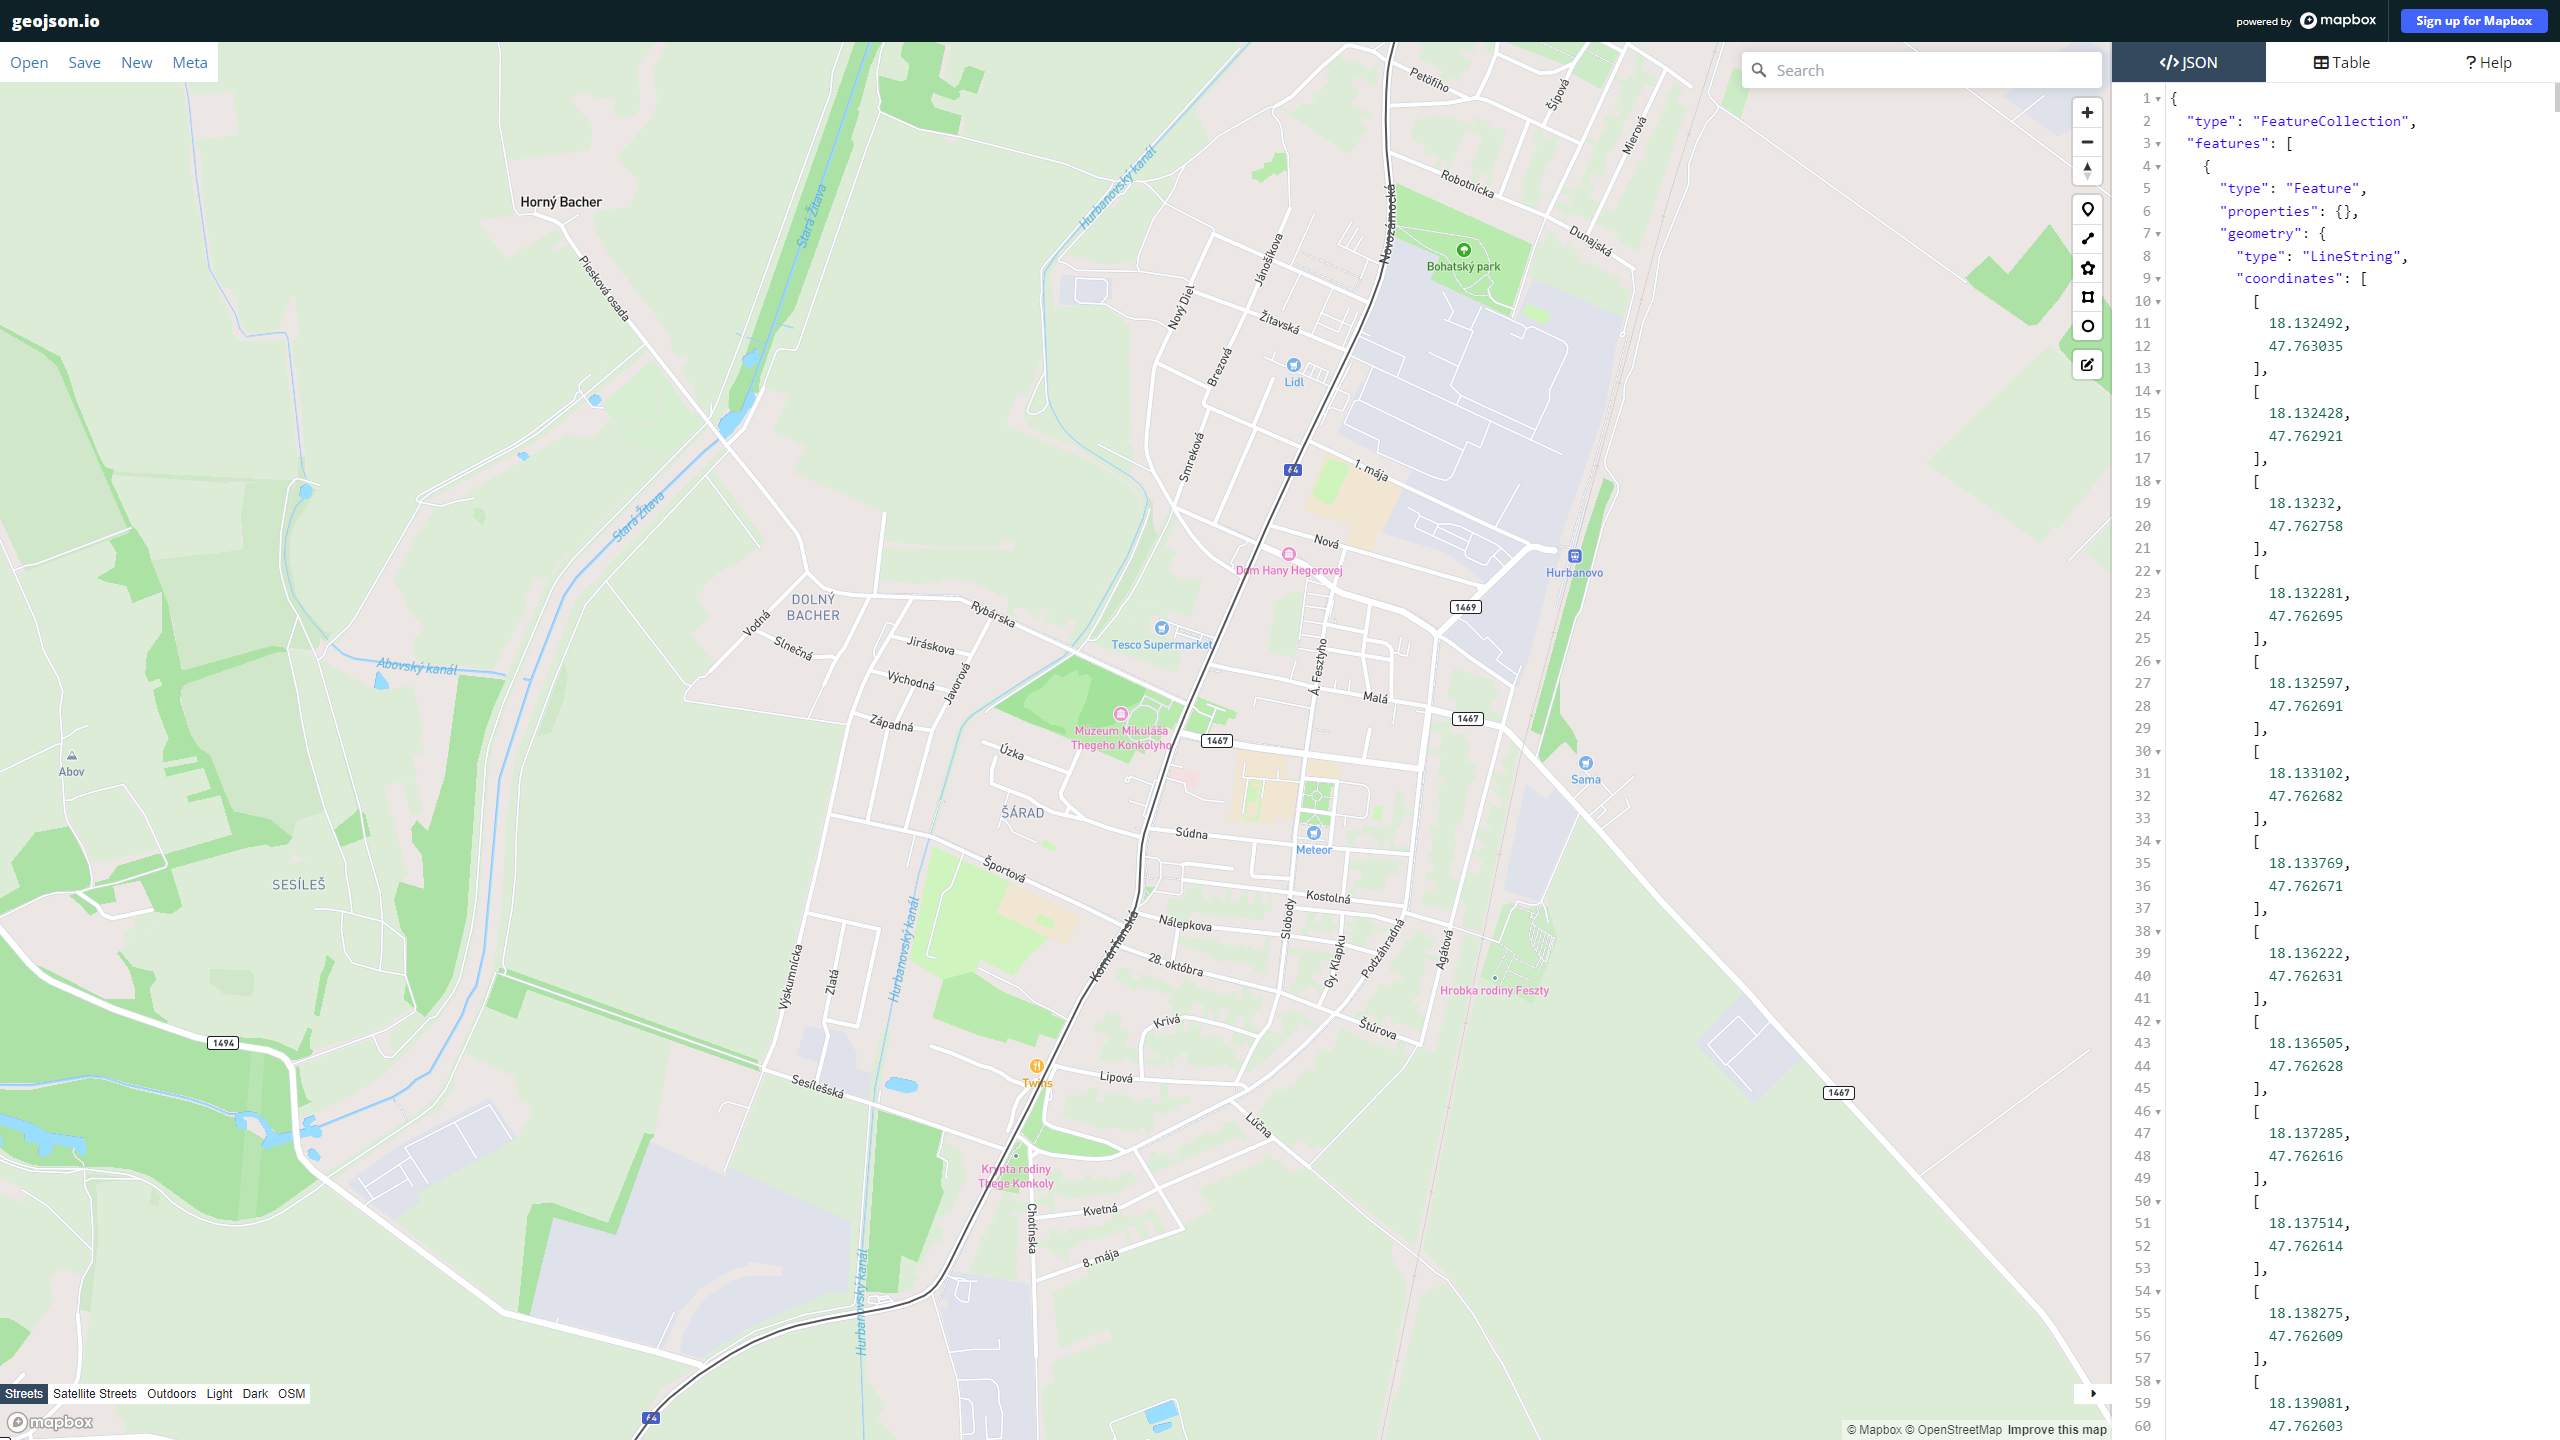
\includegraphics[width = \linewidth]{img/geojson.png}
    \caption{Prostredie Geojson.io}
\end{figure}
\subsection{Kepler.gl}
\indent \indent \textit{Kepler.gl} je open-source nástroj na geopriestorovú analýzu vyvinutý spoločnosťou \textit{Uber}. Ide o webovú aplikáciu, ktorá používateľom umožňuje vizualizovať a skúmať rozsiahle súbory geolokačných údajov. Kepler.gl je údajovo agnostický a dokáže vykresliť milióny bodov reprezentujúcich tisíce ciest, čo z neho robí výkonný nástroj na priestorovú analýzu a vizualizáciu. Je postavený na platforme \textit{deck.gl WebGL} na vizualizáciu údajov a možno ho okamžite použiť z webového prehliadača bez toho, aby ste museli čokoľvek inštalovať. Kepler.gl je v Uberi široko používaný na podporu pokročilých geopriestorových analýz inžiniermi, analytikmi a dátovými vedcami\cite{kepler1}\cite{kepler2}\cite{kepler3}.
\begin{figure}[H]
    \centering
    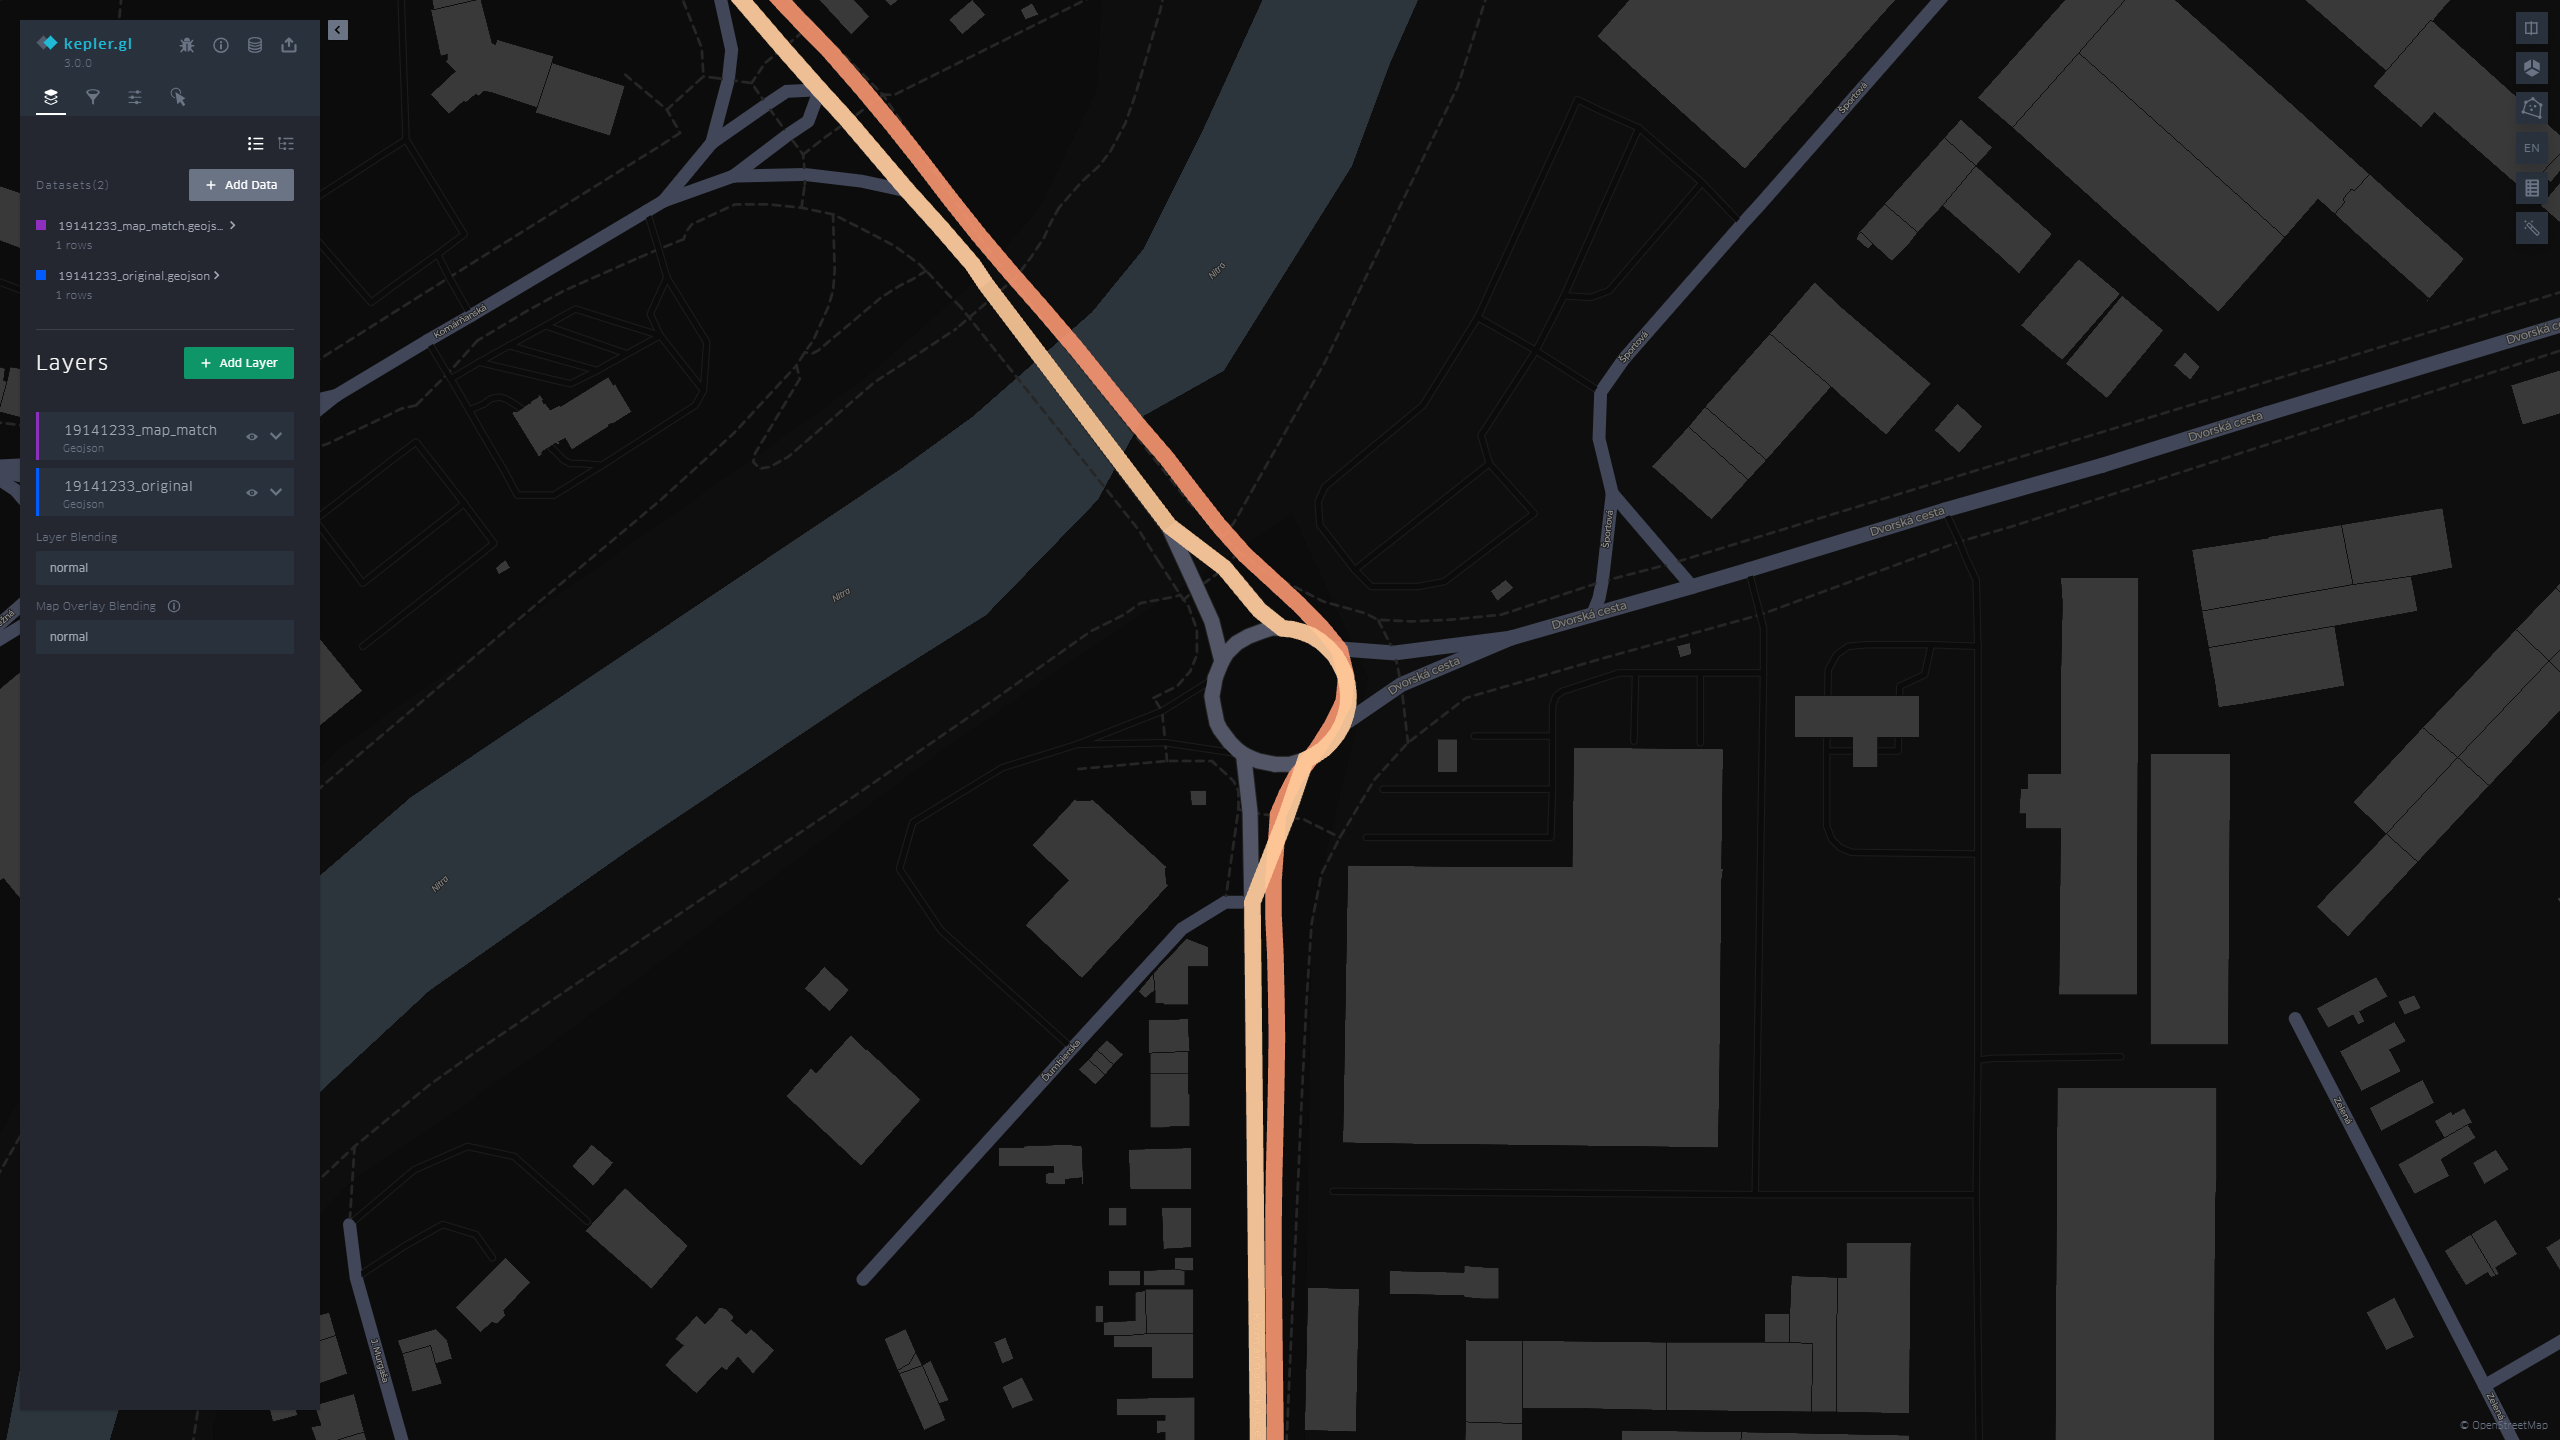
\includegraphics[width = \linewidth]{img/kepler.png}
    \caption{Prostredie Kepler.gl}
\end{figure}
\subsection{Express (Node.js)\label{section:express}}
\indent \indent \textit{Express} je backend aplikačný framework na vytváranie serverovej časti webových aplikácii. Je vydaný ako bezplatný softvér s licenciou MIT. Dá sa nazvať štandardným serverovým frameworkom pre \textit{Node.js}\cite{express}. Jeho prvá verzia, aspoň podľa histórie \textit{Githubu}, bola dňa 22. Mája 2010. Prvá vydaná verzia bola 16. Novembra 2010\cite{express_history}. Express je napísaný v Javascripte a beží na Node.js platforme. \\Výhody Express\cite{express_adv_dis}:
\begin{itemize}
    \item \textbf{Jednoduchý na použitie}: Express je účínná a užívateľsky prívetivá platforma. Má intuitívnu API a jednoduchú štruktúru. Umožňuje zostaviť aplikáciu len pomocou pár riadkov kódu, ktoré majú priamu a minimalistickú syntax. 
    \item \textbf{Veľká komunita}: Mnoho vývojárov používa tento framework, takže je veľmi populárny a existuje množstvo návodov, pomôcok a fór, kde sa dá obrátiť pri probléme pri vývoji. Taktiež má množstvo rozšírení, middleware a ďalších nástrojov, ktoré môžu byť integrované do aplikácií. 
    \item \textbf{Spraovanie HTTP požiadaviek}: Vďaka jednoduchému a flexibilnému spôsobu definovaniu ciest pre rôzne \acrshort{http} požiadavky môžeme ľahko určiť ako bude naša aplikácia reagovať a pracovať s dátami podľa našich potrieb.
    \item \textbf{Škálovateľnosť}: Express je ľahko škálovateľný, takže pri vhodnom návrhu aplikácie môžeme efektívne spracovať aj veľké množstvo požiadaviek. 
\end{itemize}
Nevýhody Express\cite{express_adv_dis}:
\begin{itemize}
    \item \textbf{Bezpečnosť}: Bolo ohlásených mnoho bezpečnostných problémov, ako napríklad vzdialené spustenie kódu pomocou \textit{ejs} modulu alebo častný \textit{denial of service} pri čersstvom module.
    \item \textbf{Aktualizácie}: Kedže sa tento framework stále vyvíja a zlepšuje, môže nastať, že niektoré moduly už nebudú podporované alebo sa budú používať inak ako sa očakáva. Preto je potrebné kontrolovať aktualizáie a zmeny a uistiť sa, že tieto aktualizácie neprinesú do našej aplikácie nové chyby.
\end{itemize}
Použitie Express v populárnych aplikáciách: \textit{Uber, Netflix, PayPal} a \textit{LinkedIn} \cite{express_adv_dis}.

\subsection{Visual Studio Code \label{section:vscode}}
\indent \indent \textit{Visual Studio Code} je jednoduchý, ale výkonný editor zdrojového kódu, ktorý je stiahnuteľný pre \textit{Windows, MacOS} aj \textit{Linux}. Dodáva sa so vstavanou podporou pre JavaScript, \textit{TypeScript} a Node.js \cite{vscode}. Má bohatý ekosystém rozšírení pre ďalšie jazyky. Taktiež obsahuje množstvo pluginov a rozšírení. Ponúka množstvo vývojárskych nástrojov ako integrácia gitu, debugger alebo vstavaný príkazový terminál. Bol vydaný 29. Apríla 2015 \cite{vscode_history}. Jeho hlavnými výhodami sú \cite{vscode_adv}:
\begin{itemize}
    \item Je zadarmo.
    \item Dostupný pre \textit{Windows, MacOS} aj \textit{Linux}.
    \item Je rozšíriteľný a je možné nainštalovať rozšírenia pre takmer všetky populárne programovacie jazyky. Nie je potrebné sťahovať zvlášť \textit{\acrshort{ide}} pre každý programovací jazyk, s ktorým pracujete.
    \item Pracuje rýchlejšie aj veľkým množstvom pluginov ako ostatné \acrshort{ide}. 
    \item Je bohatý na funkcie a s vhodnými nainštalovanými rozšíreniami je porovnateľný s plnohodnotnými \acrshort{ide} aj napriek tomu, že ide stále len o textový editor.
\end{itemize}
\begin{figure}
    \centering
    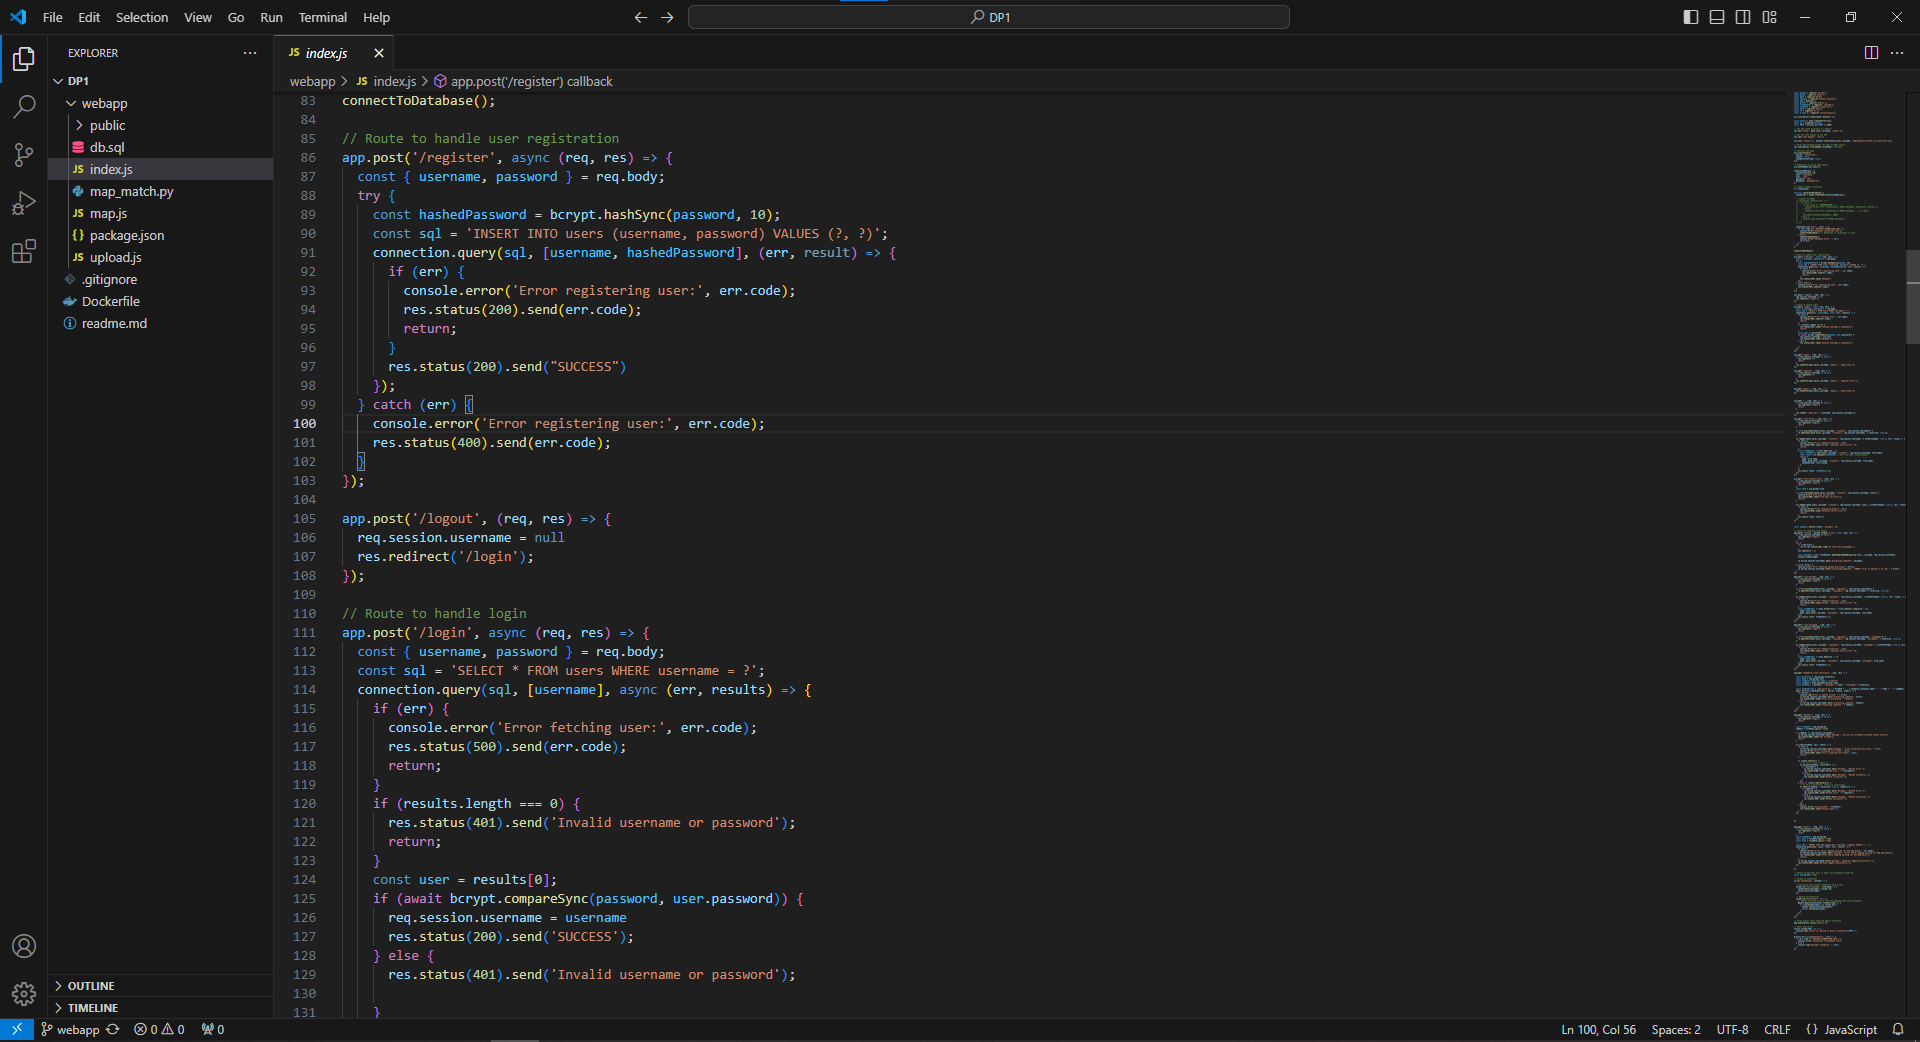
\includegraphics[width=1\linewidth]{img/vscode.png}
    \caption{Prostredie Visual Studio Code}
\end{figure}

\subsection{MySQL \label{section:mysql}}
\indent \indent Všetky softvérové aplikácie vyžadujú ako primárny zdroj údajov databázy. Databáza ukladá údaje pri vykonaní online vyhľadávania, prihlásení sa do účtu alebo dokončení transakcie, aby bolo neskôr možné tieto údaje získať. Namiesto ukladania všetkých údajov do jedného veľkého súboru, uchováva relačná databáza údaje usporiadané do tabuliek. Skutočné súbory, ktoré tvoria štruktúru databázy, sú usporiadané tak, aby maximalizovali rýchlosť. Je možné nastaviť vzťahy medzi jednotlivými údajmi 1:1, 1:N. Dátové polia môžu byť jedinečné, povinné alebo voliteľné. Databáza presadzuje tieto pravidlá, čím zaisťuje, že v prípade dobre navrhnutej databázy vaša aplikácia nikdy nenarazí na nekonzistentné, duplicitné, ojedinelé, zastarané alebo chýbajúce údaje. Časť \acrshort{sql} v \textit{MySQL} znamená \acrlong{sql}. \acrshort{sql} je najbežnejší štandardizovaný jazyk používaný na prístup k databázam. \\Výhody \textit{MySQL}\cite{mysql}:
\begin{itemize}
    \item Databáza je jednoduchá na inštaláciu, to znamená, že je vývojár nainštaluje do pár minút.
    \item Je ľahko škálovateľná. Zvládne operovať nad veľkým množstvom dát, rovnako ako obslúžiť veľké množstvo pripojení. Je preto vhodná aj pre veľké aplikácie ako \textit{Facebook}.
    \item Poskytuje mnoho bezpečnostných prkov, napríklad autentifikáciu alebo nastavenie práv pre rôznych používateľov. Vďaka tomuto sú dáta v bezpečí pred neautorizovanými používateľmi.
\end{itemize}


\subsection{Leaflet \label{section:leaflet}}
\indent \indent \textit{Leaflet} je popredná open-source knižnica napísaná v \textit{Javascripte} pre interaktívne mapy či už pre mobilné telefóny alebo počítače. Spolu má menej ako 50 \acrshort{kb} a poskytuje všetky funkcie mapy, ktoré väčšina vývojárov potrebuje\cite{leaflet}. Je jednoduchá, prehľadná a dajú sa pomocou nej jednoducho vykreslovať trasy na mapu.\\
Výhody\cite{leaflet-pros}: 
\begin{itemize}
    \item Jednoduchosť - \textit{Leaflet} je dizajnovaná pre jednoduché použitie. Je možné vytvoriť mapu jednoduchým skopírovaním kódu z \textit{QuickStart} tutoriálu \cite{leaflet-quickstart}.
    \item Dokumentácia - Dokumentácia pre \textit{Leaflet} je dobre štrukturovaná s mnohými príkladmi a návodmi.
    \item Komunita - Kedže \textit{Leaflet} je najpopulárnejšou \textit{Javascript}ovou knižnicou pre prácu s mapami a má obrovskú komunitu používateľov. Chýbajúce príklady zložitejšieho využitia sú doplnené mnohými príkladmi používateľov z komunity. ``Leaflet stackoverflow'' na \textit{Google} vyhľadávaní vráti takmer 400 tisíc výsledkov. 
    \item Flexibilita - V ponuke sú všetky funkcie, ktoré väčšina vývojárov pri práci s mapami potrebuje. V prípade potreby je možné funkcionality doplniť pluginmi.
\end{itemize} 